\begin{figure}[t]
\centering
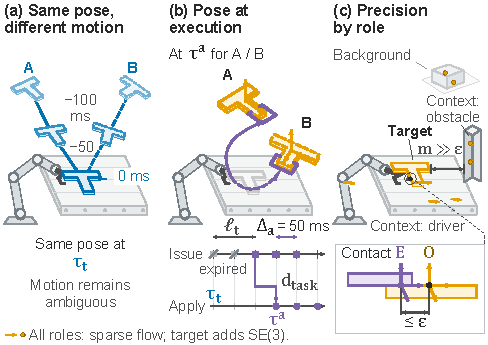
\includegraphics[width=\columnwidth]{figures/Fig3/fig3.pdf}
\caption{\textbf{作用于运动目标}（示意图）。
(a) 不同运动历史在采集时刻 $\tau_t$ 到达相同位姿。
(b) 在同一执行时刻 $\tau^{\mathrm a}$，目标的位置和朝向不同，因而需要不同指令（紫色）。
指令发出时刻从采集起每隔 $\Delta_a=50$\,ms 排列；灰色时隙在延迟 $\ell_t$ 期间过期。
保留的指令经过任务延迟 $d_{\rm task}$ 后作用于机器人，首次作用时刻为
$\tau^{\mathrm a}=\tau_t+\ell_t+d_{\rm task}$。
(c) 接触要求 $E$ 与 $O$ 在毫米级容差 $\varepsilon$ 内对齐；障碍物留下间隙
$m\gg\varepsilon$，传送带驱动目标，远处背景不影响任务。
稀疏流覆盖所有角色（箭头表示位移，圆点表示零位移），目标额外接受精细 SE(3) 监督。
位姿与延迟均为示意（$\ell_t=2\Delta_a$、$d_{\rm task}=\Delta_a$）；接触区域已放大。}
\label{fig:principles}
\end{figure}
